\section{Appendix} 

\subsection{Neural Neural Textures}

	In section \ref{sec:neural_tex}, we mentioned that neural neural textures learn better than raster neural textures. 
	Neural neural textures don't have a specific resolution: they are continuously defined over the UV domain.
	With raster-based textures, only the side of an object that currently is seen in a view is allowed to change during each update, because the gradient can't be propogated into pixels 

	The trained fourier-feature textures also exhibit less noise than its raster counterparts. 

	[[Insert figure showing the raster textures after training]]


\subsection{Unprojection Consistency Details}

	Also, the resolution of the unprojection matters:

	\begin{figure}[H]
		\begin{center}
			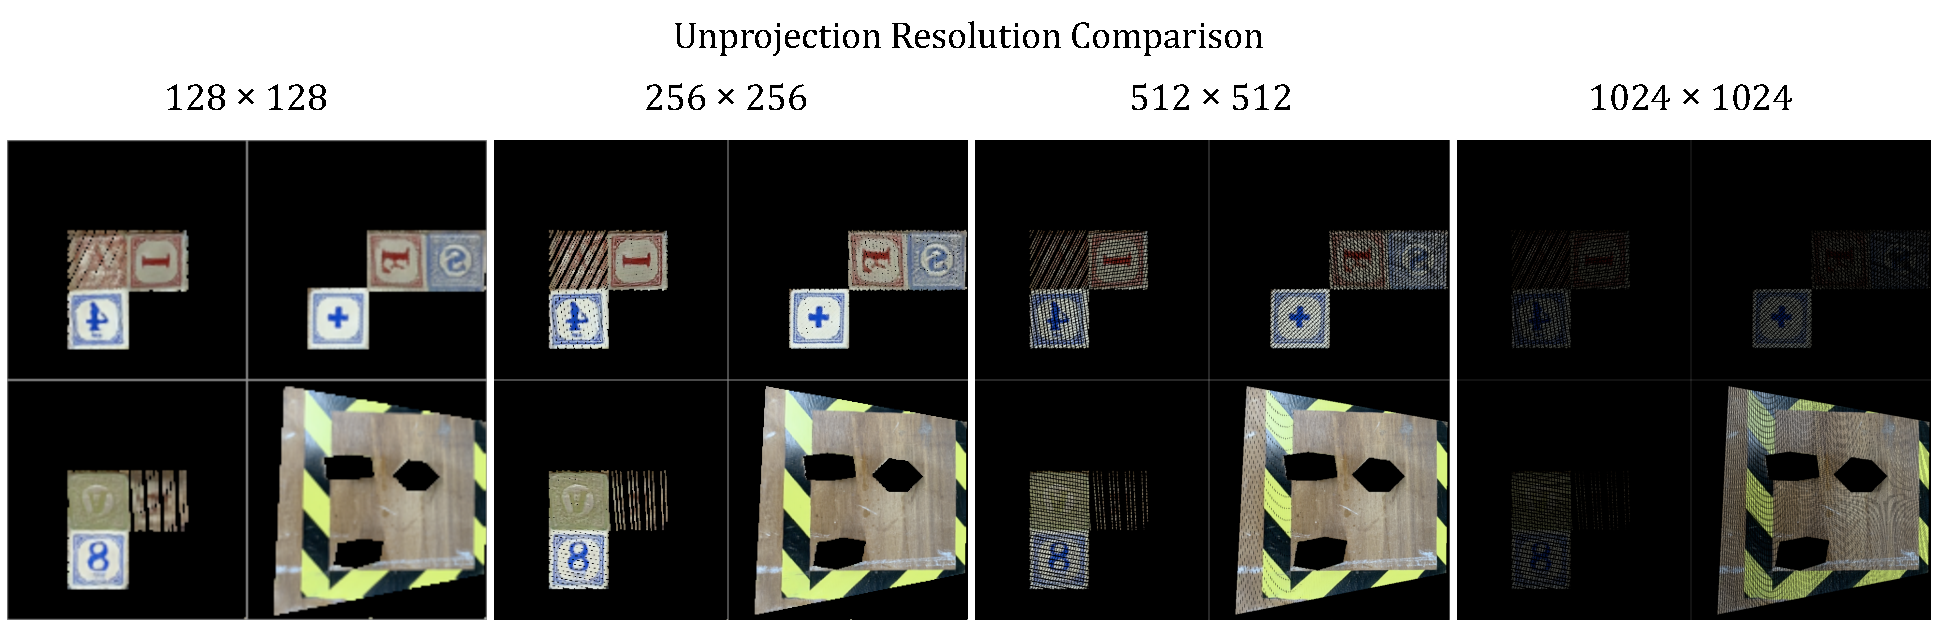
\includegraphics[width=400pt]{../images/unprojection_resolution_comparison.pdf}
		\end{center}
		\caption{
			The resolution of an unprojection matters for unprojection consistency loss. The larger it is, the more precise the alignment will be but the less likely a given UV value is to be assigned a loss greater than 0, lowering numerical instability.
		}
		\label{fig:unprojection_resolution_comparison}
	\end{figure}
	
\subsection{More Results}